\documentclass[11pt]{article}
\usepackage[letterpaper,margin={1.5cm}]{geometry}
\usepackage[utf8]{inputenc}
\usepackage[T1]{fontenc}
\usepackage[spanish]{babel}
\title{\textbf{Reporte Final \\Emergencias - 911}}
\author{Manuela Jaramillo Rendón\\
		José Manuel Vergara Álvarez\\
		}
\date{}
\usepackage{graphicx}
\begin{document}

\maketitle

\section{Acerca del proyecto}
Emergencias-llamadas 911 tiene como  objetivo   identificar y determinar que tipo de emergencias son mas frecuentes  en el condado de Montgomery,Pensilvania ubicado en Estados Unidos y además de eso, determinar cual es la probabilidad que tiene la linea de atención de emergencias (911) de recibir una llamada de ayuda para determinada causa.La implementación de este proyecto esta pensada para los diferentes organismos de respuesta a emergencias para prever el tipo de personal acorde a la necesidad del día o mes.
\section{Condado de Montgomery}
El Condado de Montgomery fundado en 1784,es uno de los 67 condados en el estado Estadounidense de Pensilvania localmente también se le denomina Montco. En el censo del 2010; la población era 799.874,convirtiendolo en el tercero con más población de Pensilvania, después de los condados de Filadelfia y el de Allegheny.
\section{Etapas de desarrollo}
El desarrollo de este proyecto se realizó en 3 etapas.
\subsection{Etapa 1: Extracción y procesamiento}
El objetivo de la primera etapa fue crear los códigos que se encargan de recuperar la información necesaria a partir de una fuente de datos externa alojada en el sitio web.
\subsection{Etapa 2: Estadística descriptiva}
Se realizó un analisis descriptivo básico de los datos de interes,sobre los cuales realizamos cálculo de la media, mínimo, máximo y desviación estandar.
Los datos seleccionados se enfocaron en el objetivo de determinar la frecuencia de las llamadas en el condado de Montogmery por día y por mes.
Los resultados obtenidos de la estadística descriptiva se muestran en la figura 1,se da resumen de frecuencias de las llamada ;se presentan más llamadas por EMS y con menor frecuenia fire y traffic ,el día en que más se presenta registros de llamadas es el  viernes  seguido del lunes ;además se observa que la hora de mayor frecuencia de llamadas esta  entre las 4 y 5 de la tarde y el mes donde se presentan mas datos es enero y después julio;también indica que la fecha con mas emergencias es  2016-01-23 . 
\\ 
\\ 
Se realizaron los promedios de las llamadas por tráfico al día(Figura 2),promedio de llamadas al mes(Figura 3),promedio de alergias mensuales(Figura 4),promedio de víctimas fatales por mes(Figura 5).
\\ 
\\ 
\\ 
\\ 
\\ 
\\ 

\begin{figure}[htp]
\centering
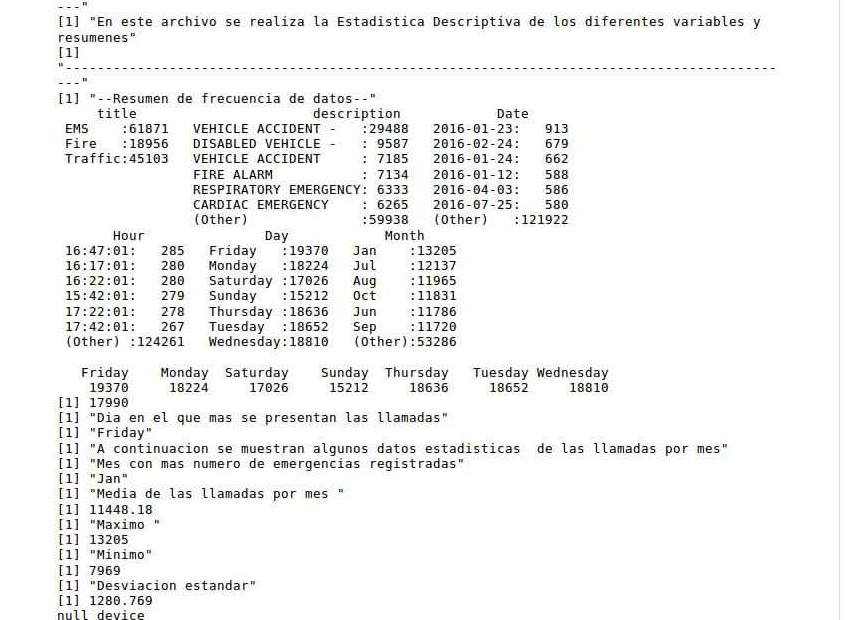
\includegraphics[scale=0.80]{/home/manuela/Emergencias_911_/Codigo/Estadistica_descriptiva.jpg}
\caption{}
\label{}
\end{figure}
\begin{figure}[htp]
\centering
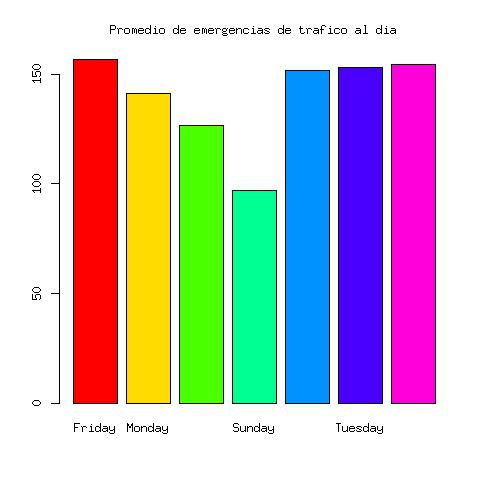
\includegraphics[scale=0.70]{/home/manuela/Emergencias_911_/Codigo/prom_trafico_al_dia.jpg}
\caption{}
\label{}
\end{figure}
\begin{figure}[htp]
\centering
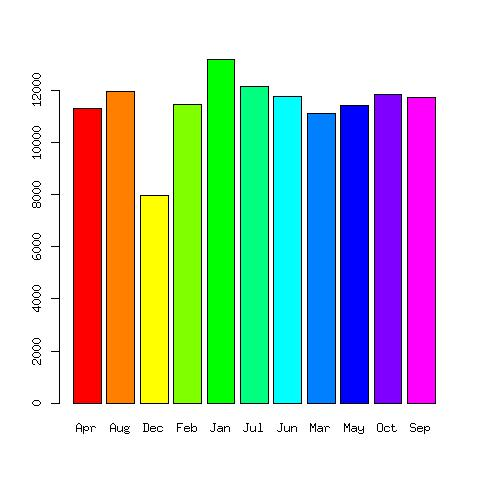
\includegraphics[scale=0.60]{/home/manuela/Emergencias_911_/Codigo/prom_llamadas_por_mes.jpg}
\caption{}
\label{}
\end{figure}
\begin{figure}[htp]
\centering
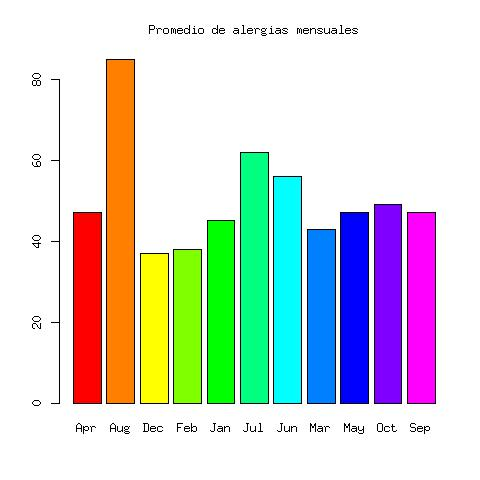
\includegraphics[scale=0.70]{/home/manuela/Emergencias_911_/Codigo/Alergias_mes.jpg}
\caption{}
\label{}
\end{figure}
\begin{figure}[htp]
\centering
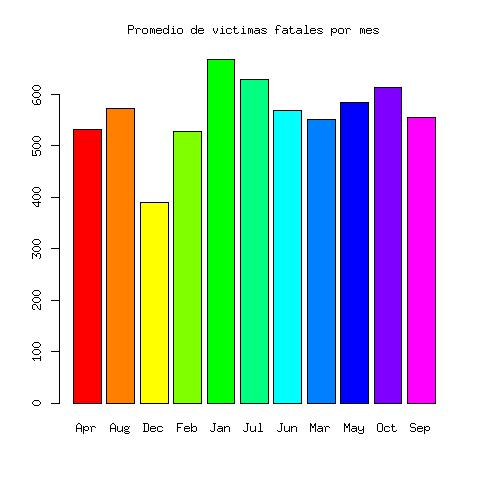
\includegraphics[scale=0.50]{/home/manuela/Emergencias_911_/Codigo/victimas_fatales_mes.jpg}
\caption{}
\label{}
\end{figure}
\
\subsection{Etapa 3: Estadística Inferencial}
\
En esta etapa se realiza un análisis  de los datos con el fin de aproximar una curva al  comportamiento de las variables y asi poder hacer una predicción del número de llamadas al día.\\
\\
EMS(Figura 6)
La curva de ajuste al promedio de llamadas por día de EMS(Emergencias de salud).Como se observa en la gráfica el numero de llamadas por día oscila aproximadamente entre 150 y 200.
\\
\\
Fire(Figura 7)
La curva de ajuste al promedio de llamadas por dia de emergencias relacionadas al fuego esta el rango de 50 y 80 mostrando  menor número de llamadas comparado con las de EMS.
\\
\\
Tráfico(Figura 8)
El promedio de llamadas al dia por emergencias de tráfico esta entre 100 y 200,observamos que las llamadas mas frecuentes son las de EMS seguidas de tráfico y fuego.
\begin{figure}[htp]
\centering
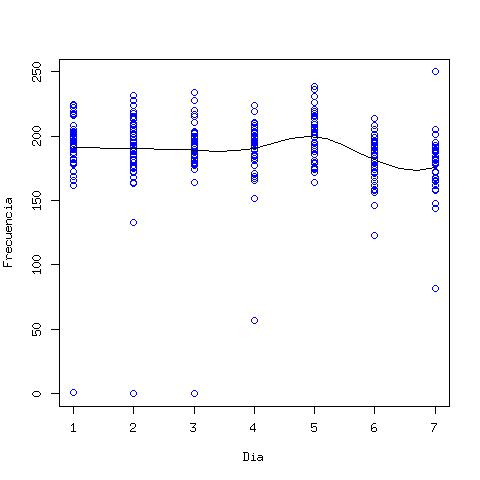
\includegraphics[scale=0.70]{/home/manuela/Emergencias_911_/Codigo/EMS.jpg}
\caption{}
\label{}
\end{figure}

\begin{figure}[htp]
\centering
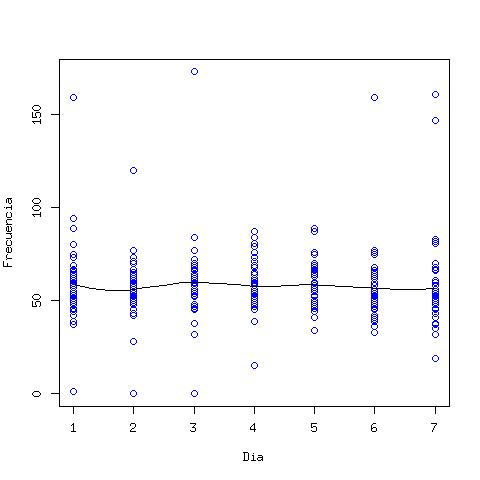
\includegraphics[scale=0.65]{/home/manuela/Emergencias_911_/Codigo/Fire.jpg}
\caption{}
\label{}
\end{figure}
\begin{figure}[htp]
\centering
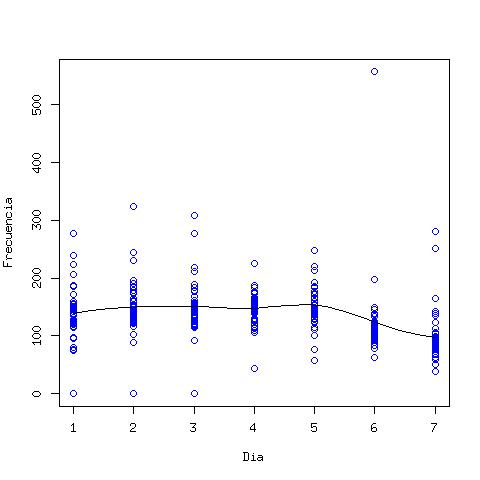
\includegraphics[scale=0.65]{/home/manuela/Emergencias_911_/Codigo/Traffic.jpg}
\caption{}
\label{}
\end{figure}
\end{document}
